\section{Background}\label{sec:background}

We begin by summarizing the necessary background information. We refer the reader
to~\cite{HatcherAlgebraic02, EdelsbrunnerComputational10} for additional background in algebraic
topology,  and computational topology respectively.

Given a topological space, $X$ and an integer $k \in \Z$, we denote the
\emph{$k^{th}$ homology group} as $H_k(X)$. We assume $\Z/2\Z$
coefficients for this paper.

\begin{defn}[Homological Critical Values]
    Let $X$ be a topological space, $f:X \rightarrow \R$ a function. We
    call~ $a\in \R$ a \emph{homological critical value} if there exists $k \in \Z$ and
    $\delta > 0$ such that for all $0 < \varepsilon < \delta$, the linear map
    $H_k(f^{-1}(-\infty, a-\varepsilon)) \rightarrow H_k(f^{-1}(-\infty,
    a+\varepsilon))$ induced by the inclusion of sublevel sets is not an isomorphism.
\end{defn}

In other words, the homological critical values are the values at which the
homology of the sublevel sets change. For Morse functions over $\R$, these points are exactly the heights of the local extrema of $f$ \cite{MilnorMorse63}.

\begin{defn}[Tameness]
    Let $X$ be a topological space. A function $f: X \rightarrow
    \R$ is \emph{tame} if it has a finite number of homological critical values
    and the homology groups $H_k(f^{-1}(-\infty, a])$ are finite for every $a
    \in \R$.
\end{defn}

\begin{defn}[Nicely Tame Functions]
    Let $X \subset \R$ be a topological space. A function $f: X \rightarrow \R$
    is \emph{nicely tame} if $f$ is tame, continuous, and for each critical
    value $y$, the preimage $f^{-1}(y)$ is a finite set.
\end{defn}

We work with nicely tame functions on a closed interval, which we denote by
\mbox{$C\subset \R$}.  Hence, the zeroth dimensional homology group (which captures
connectedness) is the only nontrivial group.

%%%%%%%%%%%%%%%%%%%%%%%%%%%%%
\subsection{Persistence Diagrams from Sublevel Set Filtrations}

Persistent homology tracks how homological  features evolve in a nested sequence
of topological subspaces.  We work with a specific case of persistent homology that
encodes the changes of the connectedness of sublevel sets of a function~$f: X
\rightarrow \R$ as the height (domain) parameter ranges from~$-\infty$ to~$\infty$. This
information is encoded in a persistence diagram and encodes the prominence of
the local extrema of $f$. Persistent homology is a general mathematical framwork
and we only provide the definitions necessary for our results here;
see \cite{EdelsbrunnerComputational10,PereaA19} for more detailed
introductions to persistence.

A \emph{filtration} of a topological space $X$ is a nested family of subspaces
$(X_r)_{r\in T}$ where $T \subseteq \R$,
such that for all $r, s \in T$ where $r\leq s$, we have $X_r \subset X_s$, and $\bigcup_{r \in T} X_r = X$. For
$f: X\rightarrow \R$, the sequence of all such \emph{sublevel sets} $f^{-1}(-\infty, r]$ ordered by inclusion and indexed
by $\R$ is the \emph{sublevel set filtration}.

Given a topological space $X$ and $f: X\rightarrow \R$, we study the zeroth
dimensional homology of sublevel sets~$H(f^{-1}(-\infty, r])$. The topological
relationships between homology groups of sublevel sets are encoded in a
persistence diagram.

\begin{defn}[Persistence Diagram $D(f)$]\label{def:pd}
    Let $f: C\rightarrow \R$ be a nicely tame function. Let
    \mbox{$\overline{\R}=\R \cup \{-\infty, \infty\}$}. The \emph{persistence diagram}
    $D(f)$ is the multiset
    set of points in $\overline{\R}^2$ such that the point~$p = (r,
    s)\in\overline{\R}^2$ is included with multiplicity, 
    $$
        \mu(p) := \lim_{\varepsilon \to 0} \left( \beta(r,s) -
        \beta(r-\varepsilon,s)-\beta(r,s+\varepsilon)+\beta(r-\varepsilon,s+\varepsilon)
        \right) 
    $$
    where $\beta(r,s)$ is the
    rank of $H(f^{-1}(-\infty, r]) \to H(f^{-1}(-\infty, s])$. We set $p \in D(f)$ if, and only if, $\mu(p) >0$. 
    \end{defn}

The persistence diagram summarizes the homology
groups as the height parameter ranges from~$-\infty$ to~$\infty$.  Each
persistence point $p=(b,d)\in D(f)$ is called a \emph{birth-death pair}.
Colloquially speaking, each $p$ represents a unique generator of the
homology groups of the sublevel sets of $f$ that is `born' at parameter~$b$ and
`dies' going into parameter $d$. If the function values of the local
extrema are unique for a function over~$\R$,
then we have a one-to-one correspondence between
persistence points and the local minima of $f$,
where $(b,d)$ corresponds to the local minimum $(t,f(t)=b)$.
In the event that the values of several minima are the same, this correspondence is not unique. However, a unique
correspondence can be induced by fixing an order on the local minima (e.g.,
 the domain coordinates) and using
that ordering to break ties.

For a multiset $A$, we write $\size{A}$
for the \emph{total multiplicity of $A$} i.e., $\size{A} = \sum_{p \in
A} \mu(p)$. \figref{PD} gives an example of a function and its persistence
diagram from a sublevel set filtration.

A key observation is that each point in $D(f)$ has a birth
coordinate that is equal to the height of a local minimum and a death coordinate
that is equal to the height of a local maximum, except for the point where the
death coordinate is $\infty$. 
We call the unique point in $D(f)$ with a death coordinate of $\infty$
the \emph{essential connected component}. From the key observation it follows that  if
$t$ does not represent the essential component, then there exists a local
maximum $(t', f(t'))$
such that $(f(t),f(t')) \in D(f)$.
In this case, $f(t')$ is the height at which the connected
component of~$f^{-1}(-\infty, f(t')]$ containing $t$ merges with another
connected component of the sublevel set $f^{-1}(-\infty, f(t')]$ represented by
a local minimum $s$ where $f(s) < f(t)$.\footnote{The choice of pairings in
$D(f)$ follows the Elder Rule (See section 7.1 of
\cite{EdelsbrunnerComputational10}): when two sublevel sets
merge together, the connected component born at the lowest height `continues',
while the other connected component `dies'. In the case where both connected
components are born at the same height, we arbitrarily choose to continue the
connected component that occurs first in the domain.} We call $f(t')$ the
\emph{merge height of $t$}.

\begin{figure}[htp]
    \centering
    {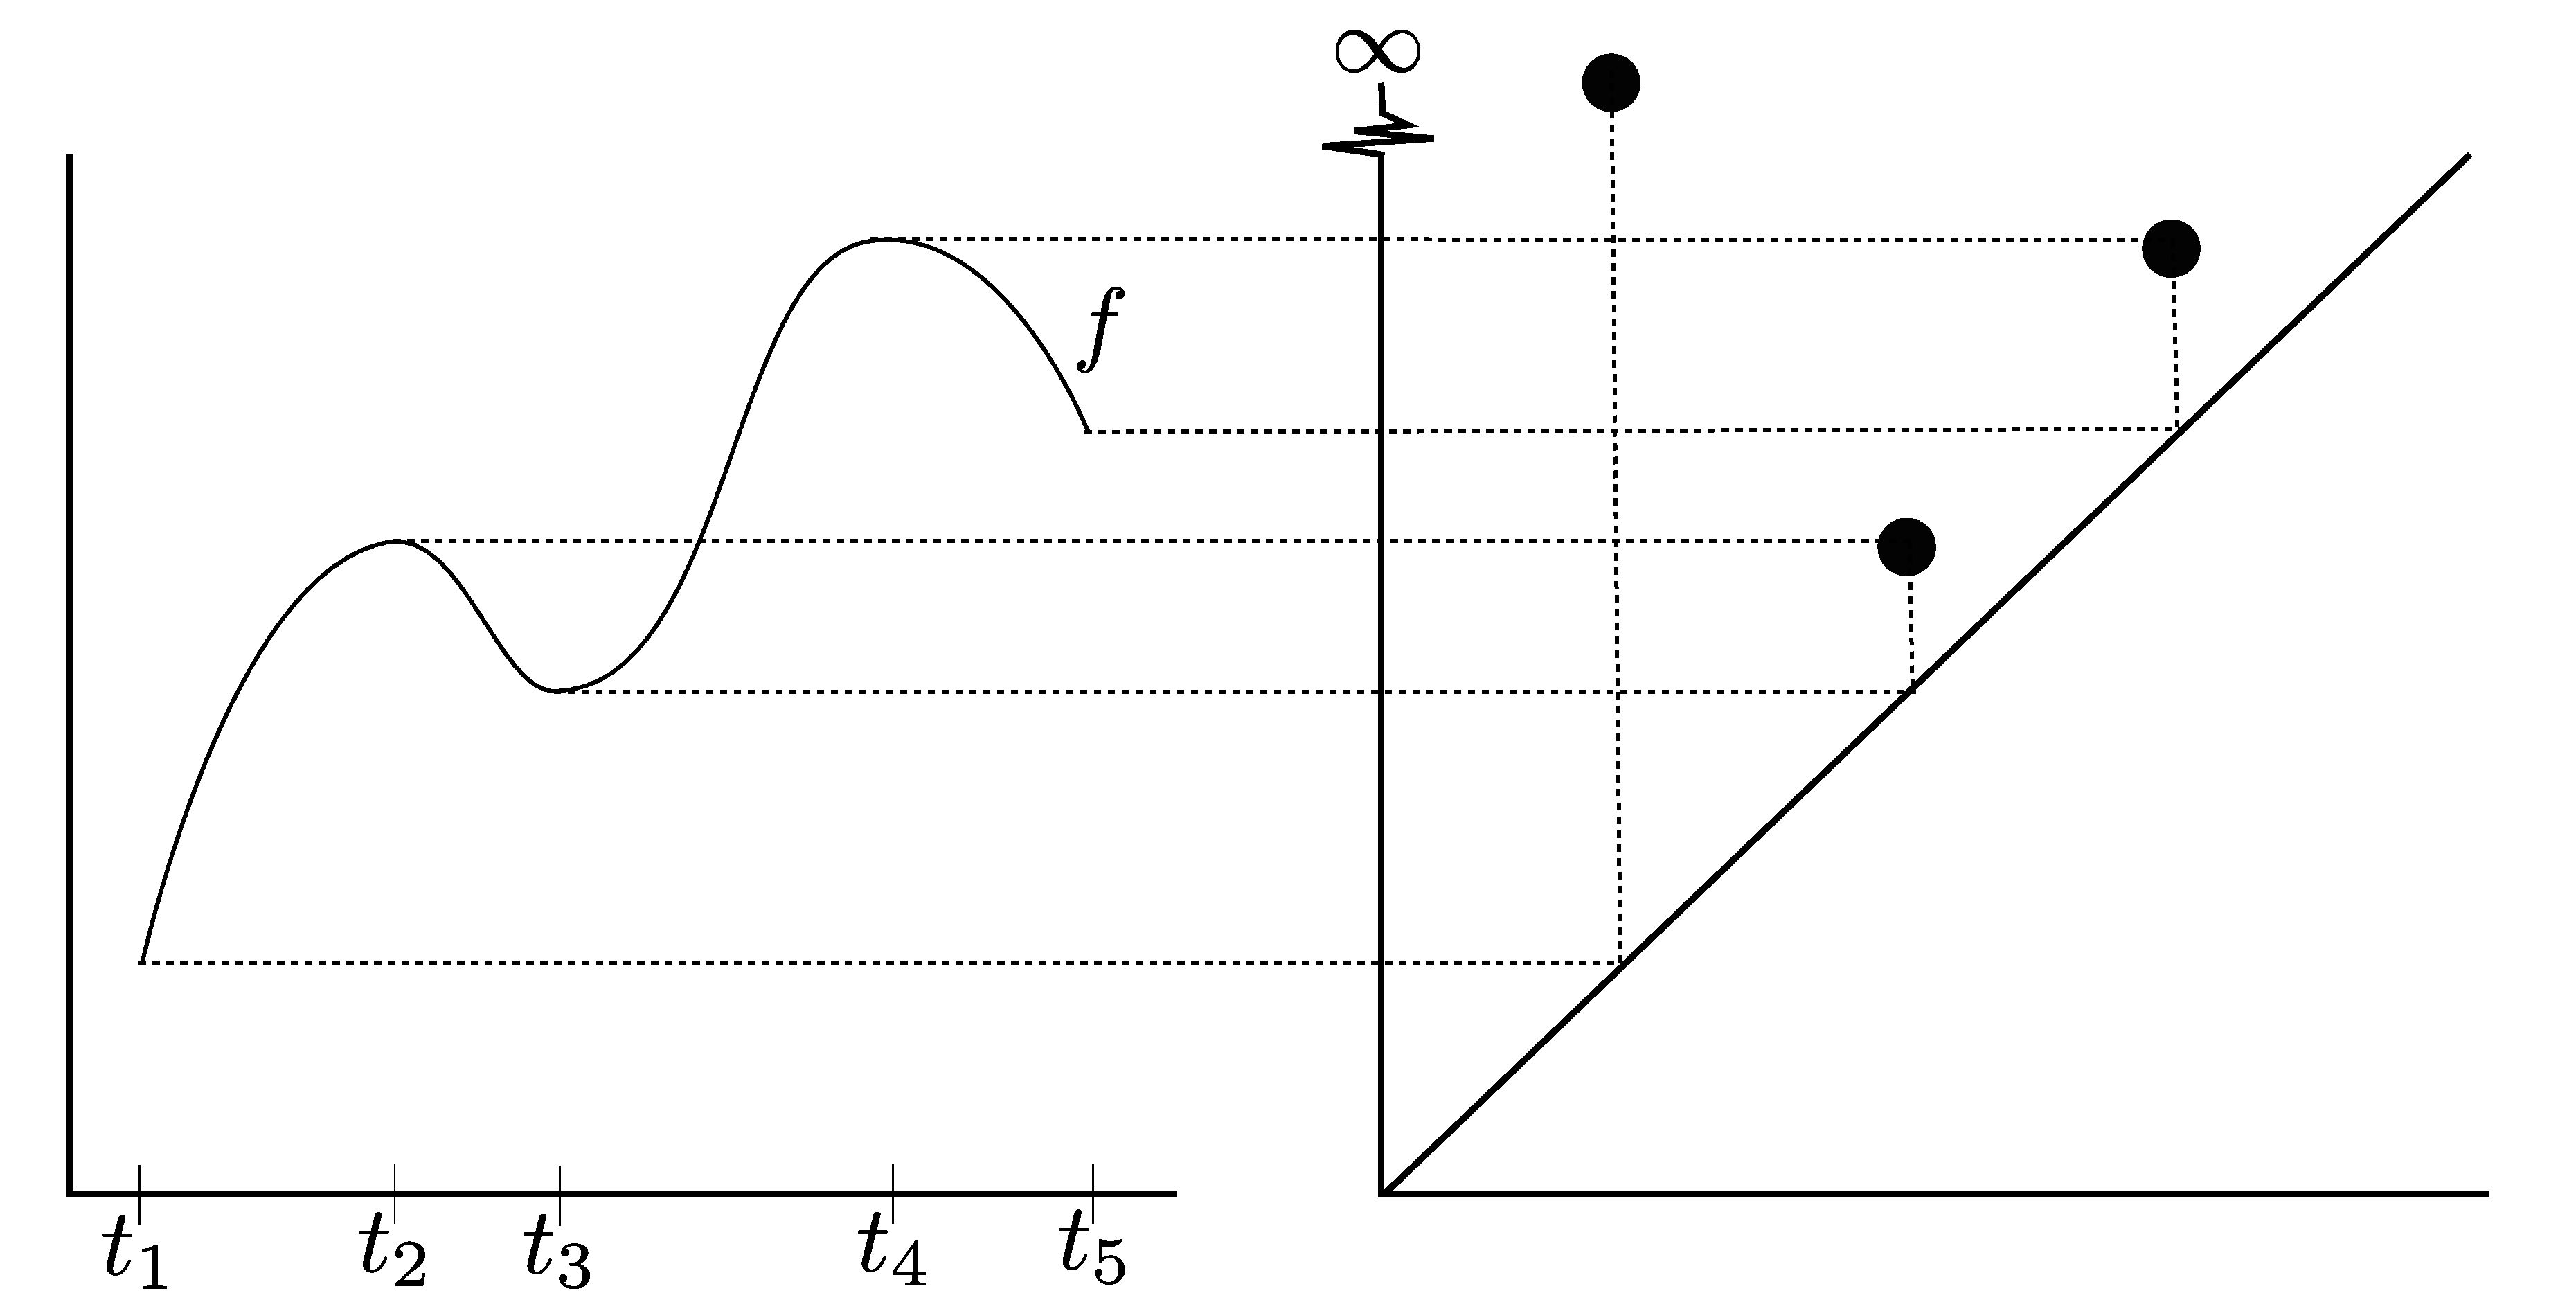
\includegraphics[width=.7\textwidth]{images/nodelife.pdf}} \\
    \caption{Left. A nicely tame function, $f:[a_1,a_2]\rightarrow \R$. Right. Persistence diagram of $f$, $D(f)$
	obtained from a sublevel set filtration of $f$.  The set
	$D(f)$ is $\{(f(t_1), \infty), (f(t_3), f(t_2)), (f(t_5), f(t_4))\}$. The first coordinate of each point in $D(f)$ is the height of a local minimum, while the second coordinate is the height of a local maximum or $\infty$.  }
    \label{fig:PD}
\end{figure}

%%%%%%%%%%%%%%
\subsection{Node Lives}
\label{sec:node-lives}

Given a function $f \colon C \to \R$ and the domain coordinate $t$ of a local
extremum, any continuous function $g\in N_\varepsilon(t)$ is guaranteed to have 
the same type of extremum in the interval~$\varphi^f_{\varepsilon}(t)$. At some
value of $\varepsilon$, however, this is no longer guaranteed.
We use the persistence diagram $D(f)$ to assist us with understanding when this
occurs.

\begin{defn}[Birth-Death Pairing Map]
   % \brittany{I added this def. back in b/c I didn't have time to remove all of  tis references}
    Let $C \subset \R$ and $f:C\rightarrow \R$ be a nicely tame function.
    Let~$\{t_i\}_{i=1}^n$ be the
    set of domain coordinates of the local minima of $f$. Define the
    \emph{birth-death pairing map} to be~$\zeta_f: \{t_i\}_{i=1}^n \rightarrow \R_{>0}$ such that
    \[ \zeta_f(t_i) = \begin{cases}
        \max(f) & \text{if } t_i \text{ represents the essential component}\\
        f(t_j) & \text{ otherwise,}
    \end{cases}
    \]
    where $f(t_j)$ is the merge height of the minimum at $t_i$.
    \label{def:birth-death-map}
\end{defn}

Observe the minima for $f$ are the maxima of $-f$ and vice-versa. Additionally, the absolute difference in heights between extrema of $f$ remain the same in both $f$ and $-f$. Hence, we can study the prominence of maxima of $f$ by studying the minima of $-f$. This follows from \cite{BendichPersistent10} which discusses the symmetry between persistence diagrams computed from height filtrations that are ascending versus descending.

\begin{defn}[Persistence of Extrema]
    Let $X \subset \R$ and $f:X\rightarrow \R$ be a nicely tame function, and
    let~$(b,d) \in D(f)$.  The persistence of $(b,d)$
    is the difference between the birth and death times,
    $d-b$. Suppose $t$ is the domain coordinate such that $f(t)=b$
    and $(t,f(t))$ is the local minimum of $f$ representing the pair $(b,d)$.
    We define the \emph{persistence of the extremum}  $(t,f(t))$,
    denoted~$\pers_f(t)$, as
    \[ \pers_f(t) :=
        \begin{cases}
            \max(f)-f(t), & \text{if } (t, f(t)) \text{ is the global minimum of } f\\
            d-b, & \text{if } (t, f(t)) \text{ is a local (and not global) minimum of } f\\
            \pers_{-f}(t), & \text{if } (t, f(t)) \text{ is a local maximum of } f.\\
        \end{cases}
    \]
\end{defn}

See~\figref{nodelife} for an example of computing the persistence of local extrema.

\begin{defn}[Node Life]\label{def:nodelife}
    Let $f:C \rightarrow \R$ be a nicely tame function with a local extremum at domain coordinate $t$. The \emph{node life} of $t$ is $\pers_f(t)/2$.
\end{defn}

We sometimes omit the subscript $f$ from $\pers_f(t)$ when the function we are
computing the node life from is clear.
Proposition 2 and Corollary 1 from~\cite{BerryUsing20} states that $\varphi_\varepsilon^f(t)$ is
the smallest interval for which any nicely tame $\varepsilon$-perturbation of $f$ is guaranteed to have at least one local extremum of the same type as $t$, as long as $\varepsilon$ is less than the node life.

\begin{figure}[htp]
    \centering
    {
\includegraphics[width=.7\textwidth]{images/nodelife}}
   {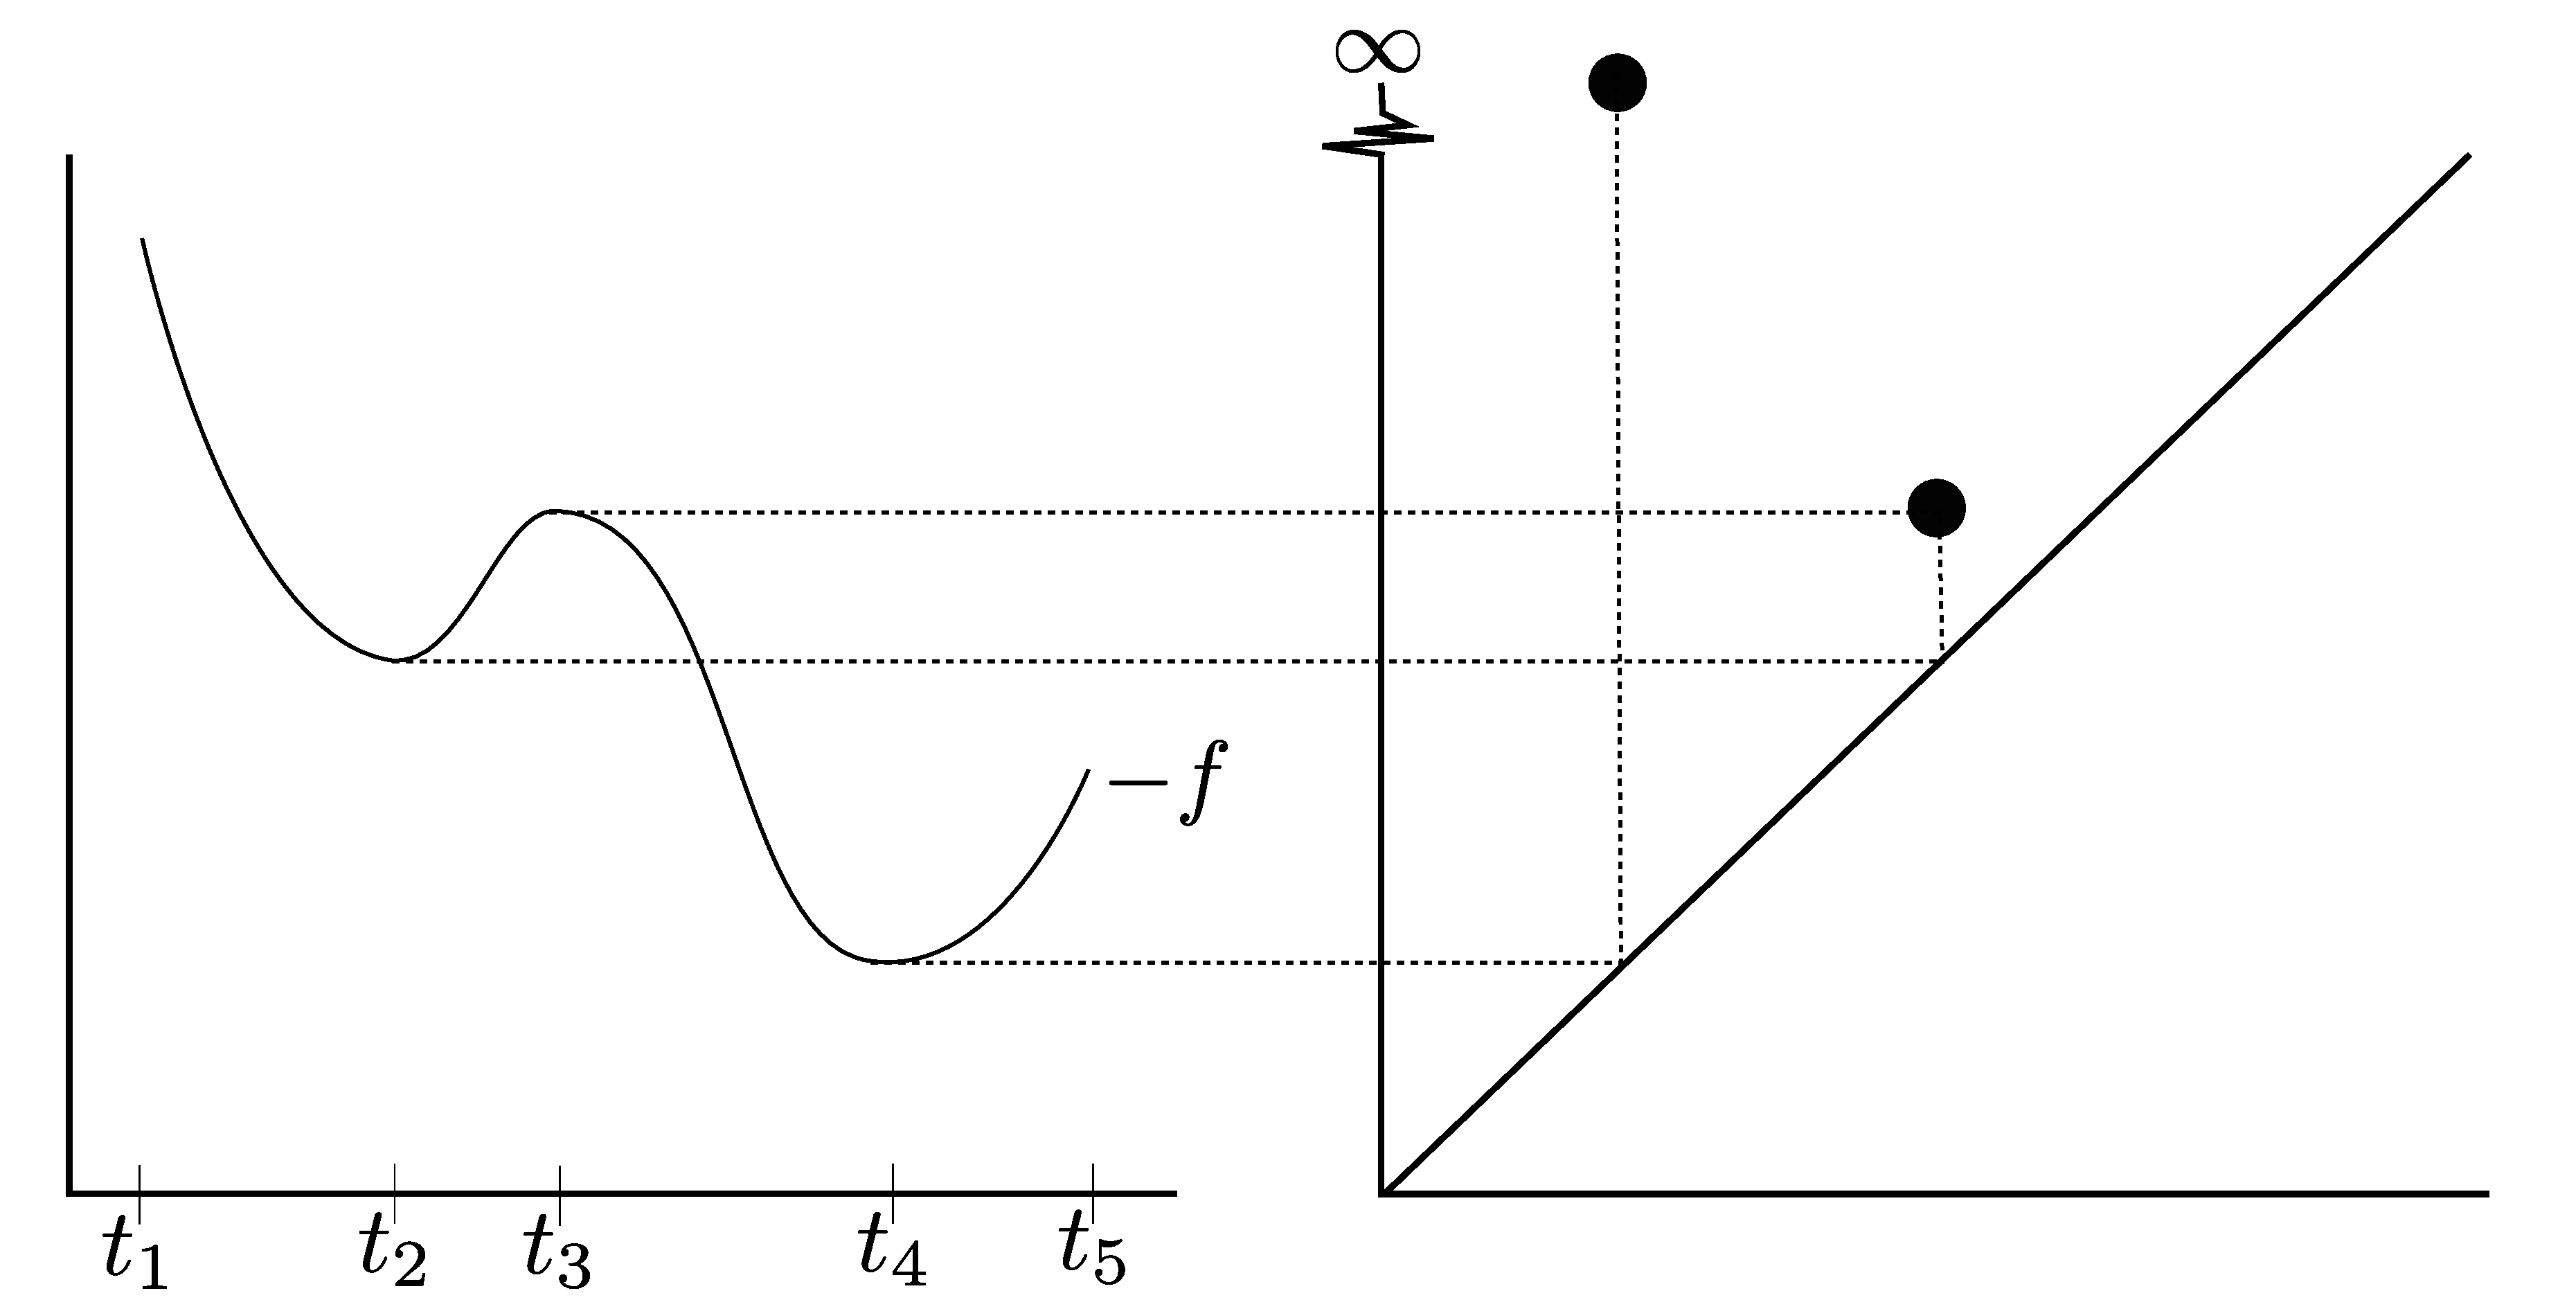
\includegraphics[width=.7\textwidth]{images/nodelife-max}}
    \caption{Top. A nicely tame function $f$ and its persistence diagram from a sublevel set filtration.
In this example, $\pers_f(t_1) = \max(f)-f(t_1)$, $\pers_f(t_3)=f(t_2)-f(t_3)$, and $\pers_f(t_5)=f(t_4)-f(t_5)$.
Bottom. $-f$ and its persistence diagram from a sublevel set filtration. Now we can compute the persistence of the local maxmima of $f$.
$\pers_f(t_4) = f(t_4)-\min(f)$ and $\pers_f(t_2)=f(t_2)-f(t_3)$.}
    \label{fig:nodelife}
\end{figure}



